\documentclass{beamer}
% \documentclass[aspectratio=169]{beamer}
\usepackage{mathpazo}

\usefonttheme{serif}
\usefonttheme{professionalfonts}
%\setmainfont{Palatino}
\usepackage[document]{ragged2e}
\usepackage[tracking=true]{microtype}
\usepackage[scaled=0.90]{helvet}
\usepackage[scaled=0.85]{beramono}
% \renewcommand*\familydefault{\ttdefault}
\usepackage[T1]{fontenc}
\usepackage[utf8]{inputenc}
\usetheme{default}

\usepackage{listings} % For code formatting

\newcommand{\todo}[1]{{\color{red}[TODO: #1]}}

\title{\raggedright\fontfamily{phv}\selectfont{\color{black}\textls[200]{\uppercase{Analyzing Quantum Many-Body Systems with ITensor and PastaQ}}}}
% \title{SLIDES ESTILO TUFTE}
\author{\raggedright\fontfamily{phv}\selectfont{\color{black}\textls[200]{\uppercase{Matthew Fishman \\ \vspace*{0.2cm} Center for Computational Quantum Physics (CCQ), Flatiron Institute, NY \\ \vspace*{0.7cm} \texttt{\lowercase{\textls[10]{mfishman@flatironinstitute.org}}}}}}}
%  \renewcommand{\familydefault}{mathpazo}

\date{}

\setbeamerfont{frametitle}{series=\itshape}
\setbeamercolor{frametitle}{fg=black} 

\setbeamertemplate{frametitle}
{
  \vspace*{0.7cm}
    
  \insertframetitle
}


\begin{document}

\begin{frame}

  \maketitle

\end{frame}

\begin{frame}{Who am I?}

\begin{itemize}[<+->]

  \item Received my PhD from Caltech with John Preskill and Steve White in 2018.
  \item Visited Frank Verstraete and Jutho Haegeman for one year during my PhD at the University of Vienna and University of Ghent.
  \item My thesis focused on developing novel tensor network algorithms for free fermions, optimizing and contracting infinite tensor networks, etc.
  \item Joined CCQ in the fall of 2018.
  \item Associate data scientist at CCQ, lead developer of ITensor and co-developer of PastaQ with Giacomo Torlai.
  \item Continuing to develop novel tensor network algorithms, with a focus on making them available as open source software.

\end{itemize}

\end{frame}

\begin{frame}{What is CCQ?}

\begin{itemize}[<+->]

\item Part of the Flatiron Institute, funded by the Simons Foundation.
\item FI is focused on supporting computational research: computers clusters, software development, algorithm development, and scientific applications.
\item 5 research centers: math, biology, astrophysics, neuroscience, and quantum.
\item Reach out to us for software needs (new features, bugs), algorithm development, etc.
\item CCQ has expertise in QMC, quantum embedding (DMFT), tensor networks, quantum dynamics, machine learning, quantum computing, quantum chemistry, etc.
\item We are hiring postdocs, full-time scientists, part-time and full-time software developers, interns, etc.

\end{itemize}

\end{frame}

\begin{frame}{What is ITensor?}

\begin{itemize}[<+->]

  \item Stands for ``Intelligent Tensor''.
  \item Started by Steve White of UCI (inventor of the DMRG tensor network algorithm) \todo{When?}.
  \item Development taken over by Miles Stoudenmire in 2011 \todo{Check this!}.
  \item I took over development in 2018, still co-developed with Miles.
  \item Originally written in C++. I led the port to Julia starting in 2019.
  \item Katie Hyatt (AWS) wrote the GPU backend in Julia.
  \item Supported by the Simons Foundation.
  \item Find out more at \myhref{https://www.itensor.org/}{itensor.org}.
  \item Paper: \myhref{https://arxiv.org/abs/2007.14822/}{arxiv.org/abs/2007.14822}.

\end{itemize}

\end{frame}

\begin{frame}{What is Julia?}

\begin{itemize}[<+->]

  \item Started in 2009, v0.1 released in 2013, v1 released in 2018.
  \item Language is very stable, ecosystem is growing very quickly.
  \item Fast like C/C++, high level features of Python, all in one language.
  \item Just-in-time compiled, garbage collected, package manager, plotting, great numerical libraries.
  \item Julia is great, you should use it.
  \item I could say more, ask me about it.
  \item Find out more at: \myhref{https://julialang.org/}{julialang.org}.

\end{itemize}

\todo{Add ITensor C++ vs. Julia benchmark plot}

\end{frame}

\begin{frame}{What is PastaQ?}

\begin{itemize}[<+->]

  \item Initiated by Giacomo Torlai while he was a postdoc at CCQ, co-developed by Giacomo and me.
  \item Quantum computing extension to ITensor.

  \begin{itemize}[<+->]

    \item Tensor network-based quantum state and process tomography. 
    \item Extensive and extendable gate definitions.
    \item Built-in and easily extendable circuit definitions.
    \item approximate circuit evolution and optimization with MPS/MPO, etc.

  \end{itemize}

  \item Find out more: \url{https://github.com/GTorlai/PastaQ.jl}

\end{itemize}

\end{frame}

\begin{frame}{When should I use tensor networks?}

\begin{itemize}[<+->]

  \item Many sites or qubits in your system: linear or log scaling in the system size.
  \item Short time evolution, or very noisy evolution.
  \item If you need very long time evolution/many layers and few qubits, use full state simultion.
    
  \begin{itemize}[<+->]

    \item ITensor and PastaQ handle this seemlessly.
    \item This is not the focus of ITensor and PastaQ at the moment, specialized libraries like Yao.jl may be faster.

  \end{itemize}

  \item In my opinion, tensor networks are the best general purpose tool we have right now for studying quantum many-body systems (while we wait for a general purpose quantum computer).
  \item Tensor networks are a common, general language for reasoning about quantum many-body systems (for example, quantum circuits).

\end{itemize}

\todo{``Quantum volume'' schematic plot.}

\end{frame}

\begin{frame}[fragile]{What are tensor networks?}

\begin{columns}

  \begin{column}[T]{0.33\textwidth}
    \centering
    Vector $V_i$ \\
    Order-1 tensor
    \begin{figure}[T]
      
\includegraphics[width=0.3\textwidth]{
        slides/assets/V.png
      }
    \end{figure}
  \end{column}

  \begin{column}[T]{0.33\textwidth}
    \centering
    Matrix $M_{ij}$ \\
    Order-2 tensor
    \begin{figure}[T]
      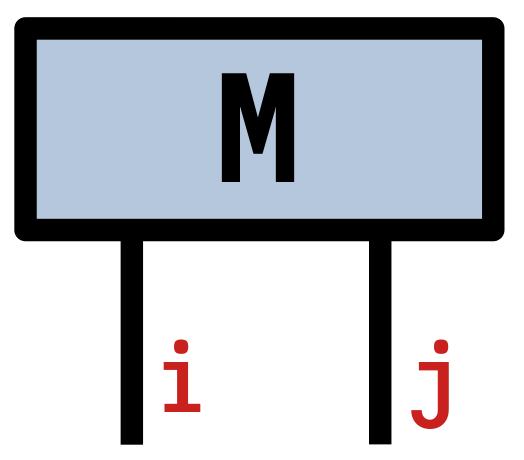
\includegraphics[width=0.5\textwidth]{
        slides/assets/M.png
      }
    \end{figure}
  \end{column}

  \begin{column}[T]{0.33\textwidth}
    \centering
    Tensor $T_{ijk}$ \\
    Order-3 tensor
    \begin{figure}[T]
      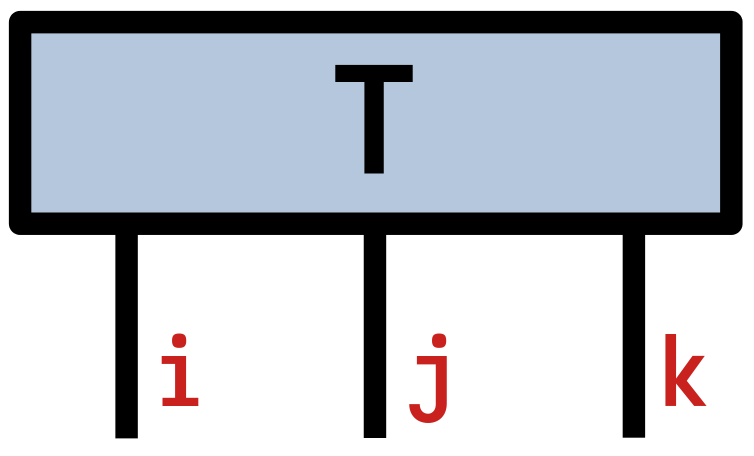
\includegraphics[width=0.7\textwidth]{
        slides/assets/T.png
      }
    \end{figure}
  \end{column}

\end{columns}

\vspace*{0.4cm}

\begin{onlyenv}<2->

\begin{columns}

  \begin{column}[T]{0.33\textwidth}
    \centering
    $\langle V|V\rangle = V_i V_i$
    \begin{figure}[T]
      
\includegraphics[width=0.7\textwidth]{
        slides/assets/VV.png
      }
    \end{figure}
  \end{column}

  \begin{column}[T]{0.33\textwidth}
    \centering
    $M|V\rangle = M_{ji} V_i$
    \begin{figure}[T]
      
\includegraphics[width=0.8\textwidth]{
        slides/assets/MV.png
      }
    \end{figure}
  \end{column}

  \begin{column}[T]{0.33\textwidth}
    \centering
    $MM = M_{kj} M_{ji}$
    \begin{figure}[T]
      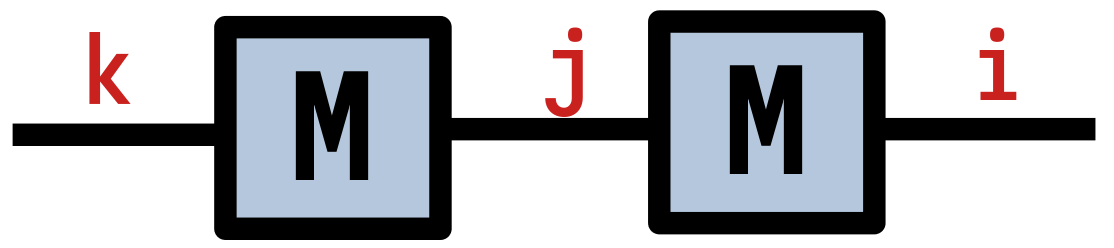
\includegraphics[width=1.0\textwidth]{
        slides/assets/MM.png
      }
    \end{figure}
  \end{column}

\end{columns}

\end{onlyenv}

\vspace*{0.4cm}

\begin{onlyenv}<3->

\centering

\begin{columns}

  \begin{column}[T]{0.5\textwidth}
    \centering
    $tr(MM) = M_{ij} M_{ji}$
    \begin{figure}[T]
      
\includegraphics[width=0.6\textwidth]{
        slides/assets/trMM.png
      }
    \end{figure}
  \end{column}

  \begin{column}[T]{0.5\textwidth}
    \centering
    $M_{ij} T_{ijk} V_{k}$
    \begin{figure}[T]
      \includegraphics[width=0.6\textwidth]{
        slides/assets/MTV.png
      }
    \end{figure}
  \end{column}

\end{columns}

\end{onlyenv}

\end{frame}

\begin{frame}{How do I install ITensor/PastaQ?}

\begin{enumerate}[<+->]

  \item Download Julia.
  \item Add ITensors.jl.
  \item Add PastaQ.jl.

\end{enumerate}

\todo{Add links, show code}

\end{frame}

\begin{frame}[fragile]{Tutorial: One-site state basics}

\begin{columns}

\begin{column}[T]{0.48\textwidth}
\begin{onlyenv}<1->
\begin{lstlisting}[language=JuliaLocal, style=julia, basicstyle=\small]
using ITensors

i = Index(2)

 \end{lstlisting}
\end{onlyenv}
\end{column}

\begin{column}[T]{0.48\textwidth}

\begin{onlyenv}<1-1>
Load ITensor \\[\baselineskip]
2-dimensional labeled \\
Hilbert space \\
(dim=2|id=510)
\end{onlyenv}

\begin{onlyenv}<2->
\begin{figure}[T]
  
\includegraphics[width=0.3\textwidth]{
    slides/assets/i.png
  }
\end{figure}
\end{onlyenv}

\end{column}


\end{columns}

\begin{columns}

\begin{column}[T]{0.48\textwidth}
\begin{onlyenv}<3->
\begin{lstlisting}[language=JuliaLocal, style=julia, basicstyle=\small]
Zp = ITensor(i)
Zp[i=>1] = 1

Zp = ITensor([1, 0], i)
\end{lstlisting}
\end{onlyenv}
\end{column}

\begin{column}[T]{0.48\textwidth}
\begin{onlyenv}<3-3>
$|Z+\rangle = \begin{bmatrix} 1 \\ 0 \end{bmatrix}$ \\[\baselineskip]
Construct from a Vector
\end{onlyenv}
\begin{onlyenv}<4>
\begin{center}
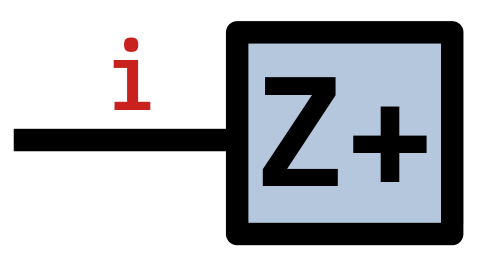
\includegraphics[width=0.3\textwidth]{
  slides/assets/Zp.png
} \\
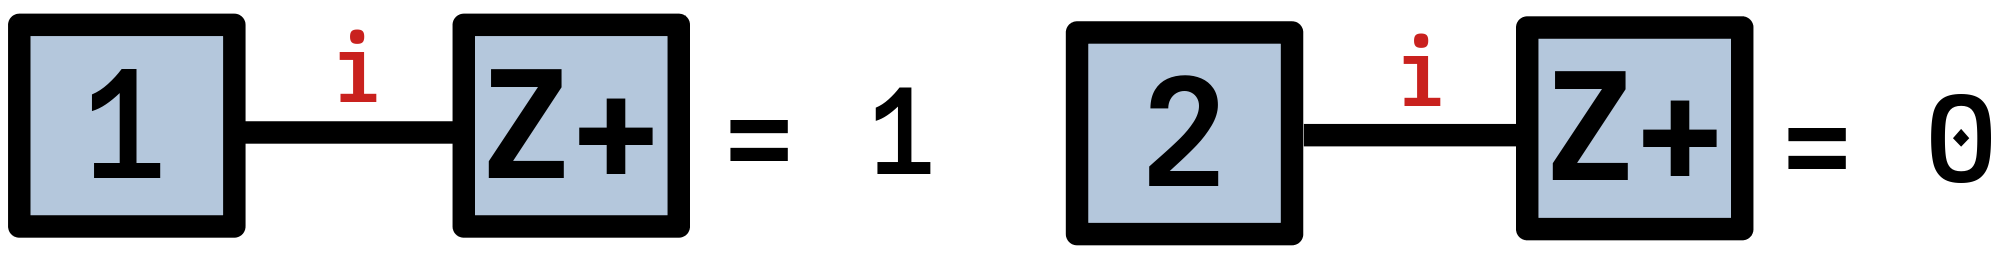
\includegraphics[width=1.0\textwidth]{
  slides/assets/Zp_elts.png
}
\end{center}
\end{onlyenv}
\end{column}

\end{columns}

\end{frame}

\begin{frame}[fragile]{Tutorial: One-site state basics}

\begin{columns}

\begin{column}[T]{0.45\textwidth}
\begin{onlyenv}<1->
\begin{lstlisting}[language=JuliaLocal, style=julia, basicstyle=\small]
Zp = ITensor([1, 0], i)
Zm = ITensor([0, 1], i)
Xp = ITensor([1, 1]/√2, i) 
Xm = ITensor([1, -1]/√2, i) 
\end{lstlisting}
\end{onlyenv}
\end{column}

\begin{column}[T]{0.6\textwidth}
\begin{onlyenv}<1-1>
$|Z+\rangle = \begin{bmatrix} 1 \\ 0 \end{bmatrix}$,
\ \ \ \ \ \ \  $|Z-\rangle = \begin{bmatrix} 0 \\ 1 \end{bmatrix}$ \\
$|X+\rangle = \begin{bmatrix} 1 \\ 1 \end{bmatrix}/\sqrt{2}$,
  $|X-\rangle = \begin{bmatrix} 1 \\ -1 \end{bmatrix}/\sqrt{2}$
\end{onlyenv}

\begin{onlyenv}<2->
\vspace*{-0.4cm}
\begin{center}
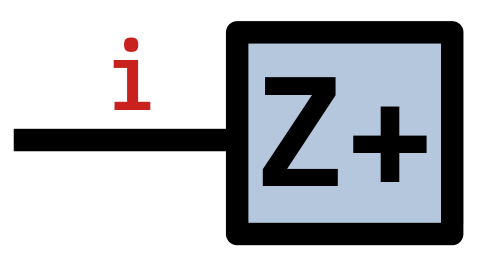
\includegraphics[width=0.3\textwidth]{
  slides/assets/Zp.png
} \ \ \ \ \ \ \ 

\includegraphics[width=0.3\textwidth]{
  slides/assets/Zm.png
} \\
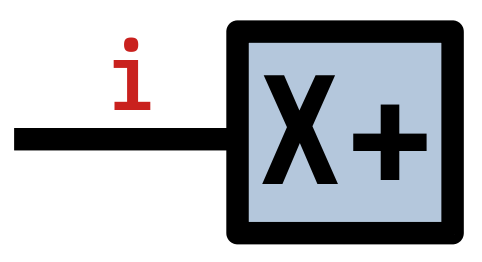
\includegraphics[width=0.3\textwidth]{
  slides/assets/Xp.png
} \ \ \ \ \ \ \ 
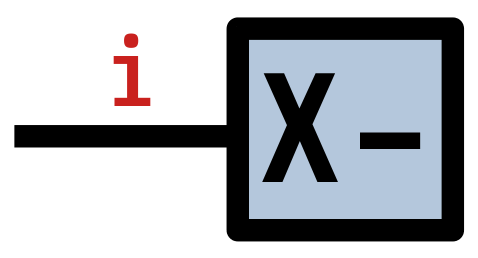
\includegraphics[width=0.3\textwidth]{
  slides/assets/Xm.png
}
\end{center}
\end{onlyenv}
\end{column}

\end{columns}

\begin{columns}

\begin{column}[T]{0.45\textwidth}
\begin{onlyenv}<3->
~\\
~\\
\begin{lstlisting}[language=JuliaLocal, style=julia, basicstyle=\small]
Xp = (Zp + Zm)/√2



dag(Zp) * Xp
inner(Zp, Xp)
\end{lstlisting}
\end{onlyenv}
\end{column}

\begin{column}[T]{0.6\textwidth}
\begin{onlyenv}<3-3>
~\\
~\\
~\\
$|X+\rangle = (|Z+\rangle + |Z-\rangle)/\sqrt{2}$ \\
~\\
~\\
$\langle Z+|X+\rangle\approx$ 1/√2 \\
$\langle Z+|X+\rangle\approx$ 1/√2
\end{onlyenv}

\begin{onlyenv}<4>
~\\
~\\
\vspace*{-0.1cm}
\begin{center}
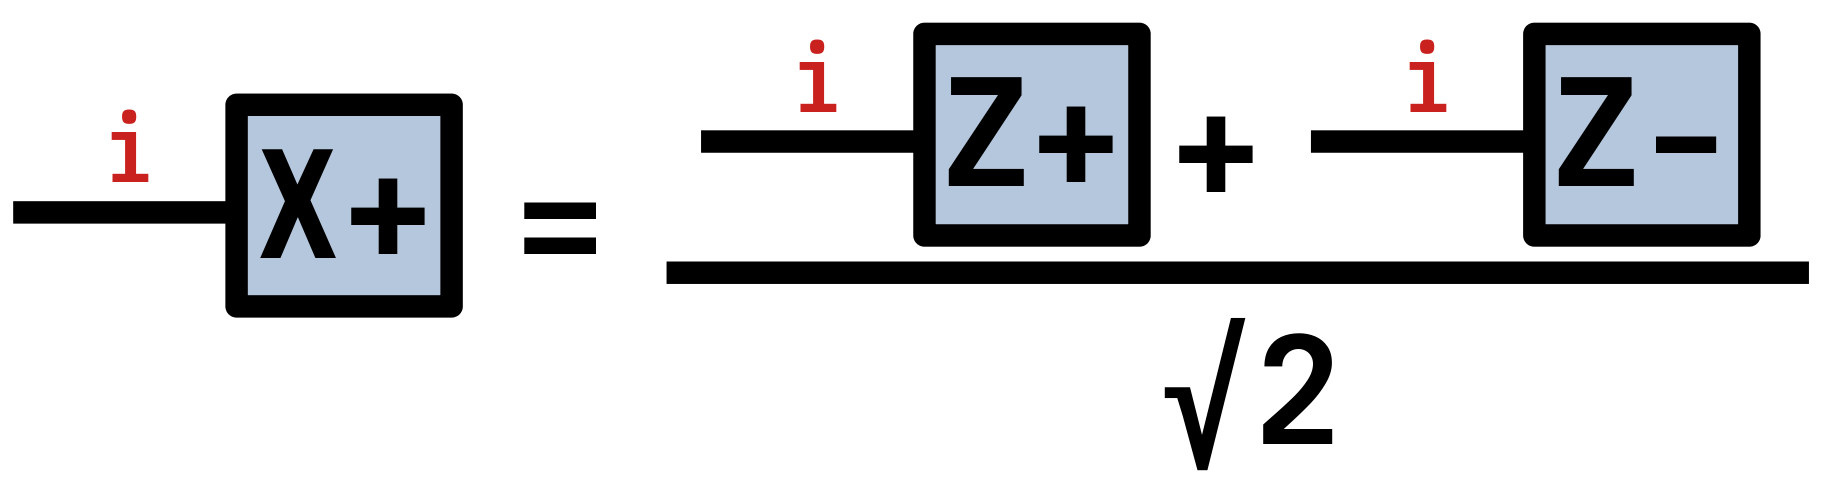
\includegraphics[width=1.0\textwidth]{
  slides/assets/Zp+Zm.png
} \\
~\\
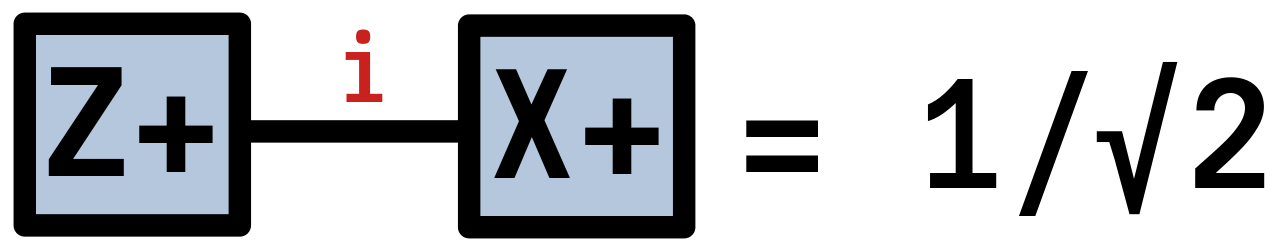
\includegraphics[width=0.7\textwidth]{
  slides/assets/ZpXp.png
}
\end{center}
\end{onlyenv}
\end{column}

\end{columns}

\end{frame}

\begin{frame}{Future directions}

\begin{itemize}[<+->]

  \item More AD, make ITensor fully differentiable (have some work to do, like tensor decompositions and general network contractions, more MPS/MPO functions. You will find bugs!).
  \item More general built-in tensor networks beyond MPS/MPO
  \item More HPC with multithreaded and multiprocessor parallelism and GPUs
  \item Many ongoing projects and directions: quantum chemistry (for example UCC), real space parallel DMRG, TDVP, and TEBD, MPO compression tools, general approximate contraction techniques for unstructured networks, contracting and optimizing general tensor networks with AD, infinite MPS and tensor network tools like VUMPS and TDVP, trying out different network topologies for noisy circuit tomography, simulation and optimization.
  \item Building general tools, looking for people with problems and code to contribute.
  \item Improved gradient optimization/preconditioners, isometrically constrained gradient optimization, etc.
  \item Automatic fermions, non-abelian symmetries.

\end{itemize}

\end{frame}


\end{document}
